\chapter{Grundlagen der Rest API}
\bauer
%Quelle: https://en.wikipedia.org/wiki/Representational_state_transfer
\section{Definition} 
REST\footcite{rest} steht für "Representational State Transfer" und wird oft zum Erstellen von interaktiven Applikationen insbesondere in der Webentwicklung verwendet. Wenn die Applikation dem Prinzip der Rest Software Architektur folgt so nennt man diese auch Restful. Die Architektur selbst beschreibt den Zugriff und die Veränderung von Ressource mit einem Zustandslosen Protokoll. Eine Rest API ist somit ein Anwendungsschnittstelle auf die durch ein Zustandsloses Protokoll zugegriffen wird.			
%Quelle: 
\section{Geschichte}
Roy Fielding schrieb im Jahre 2000 seine Dissertation über den REST-Architekturstil allerdings findet die korrekte Umsetzung erst seit dem 2014 Anklang in World Wide Web.		 	
%Quelle: https://restfulapi.net/
\section{Prinzipien}		 				 	
\subsection{Zustandslosigkeit}
Jede Anfrage auf dem Server muss sämtliche notwendige Informationen zur Ausführung der Anfrage enthalten was bedeutet das sämtliche Session Daten nur auf dem Client gespeichert werden müssen.		 	
\subsection{Caching}
Jede Antwort der Schnittstelle muss als "cachable" oder "non-cacheable" gekennzeichnet sein. Damit der Client alle Informationen für die er nicht eine erneute Anfrage an den Server schicken muss abspeichern kann. Dies erspart sowohl dem Client als auch dem Server selbst Rechenzeit.		 	
\subsection{Einheitliche Schnittstellen}
Da der Client getrennt vom Server agieren kann und nur Anfragen an diesen schickt ist es möglich mit einer Rest API eine Schnittstelle für mehrere Geräte zu entwickeln da zum Beispiel eine Smartphone App die gleiche Schnittstelle wie eine Website verwenden könnte.		 	
\subsection{Mehrschichtige Systeme}
Das System soll aus mehreren Ebenen aufgebaut werden allerdings sieht der Client selbst nur eine Schnittstelle was das Interagieren vereinfacht. Der große Vorteil liegt darin, das dieses System die Abkapslung durch eine Firewall so wie eine einfache Skalierbarkeit bietet.		 	
%Quelle: https://de.wikipedia.org/wiki/Node.js
\section{Node.js}
Node.js\footcite{nodejs} ist open-source Javascript Laufzeitumgebung welche plattformübergreifend arbeitet. Die Laufzeitumgebung wird oft dazu verwendet um Webbrowser aufzusetzen dieser läuft dann über die JavaScript-Implementierung V8. Ursprünglich wurde die Technologie für Google Chrome entwickelt das besondere An der Architektur ist, dass sie sehr ressourcensparend ist und dabei eine sehr große Anzahl von Netzwerkverbindungen gleichzeitig zulässt. Da bei der Entwicklung von Node.js ein besonderer Fokus auf Performance gerichtet wurde kommt in dieser Architektur die nonblocking I/O zum Einsatz anstatt der üblichen blocking I/O. Dies sorgt dafür, dass ein Prozess weiterarbeiten kann obwohl er noch auf Ergebnisse wartet zum Beispiel von einer Berechnung oder einer Datenbank Abfrage. 		 	
%Quelle: https://en.wikipedia.org/wiki/Node.js#:~:text=Node.js%20was%20written%20initially,and%20later%20sponsored%20by%20Joyent.
%Quelle: https://hostingtribunal.com/blog/node-js-stats/#gref
\subsection{Geschichte}
Node.js wurde ursprünglich von Ryan Dahl in 2009 entwickelt. Im Januar 2010 kam der nächste große Schritt für Node.js da zu diesem Zeitpunkt der Package Manager (npm) erschien welcher Programmiere auf der ganzen Welt eine einfache Methode gab Quellcode in Form von so genannten Packages zu entwickel und zu verbreiten. Im Juli 2011 kam die erste Node.js Version für Windows da die früheren Versionen nur unter Linux und Mac OS X veröffentlicht wurden. Im Jahr 2018 hat Node.js die 1 Milliarde Downloads. Heutzutage wird Node.js für über 20 Millionen Webseiten verwendet. 		 		
%Quellen: https://www.yuhiro.de/vorteile-und-nachteile-von-node-js/
\subsection{Vorteile}
Ein großer Vorteil der Node.js Laufzeitumgebung ist die Performanz welche geboten wird. Diese Performanz fällt besonders bei einer großen Anzahl von Verbindungen beziehungsweise Anfragen auf. Dazu kommt die Kompatibilität von Node.js sowohl zu verschiedenen Datenbanken als auch mit fast allen Frontendapplikationen da das ganze nach Rest-Prinzip aufgebaut ist. Natürlichen dürfen auch die Packages nicht außer acht gelassen werden das es über 600.000 davon gibt und jeden Tag neue hinzugefügt werden.		 		
%Quellen: https://www.yuhiro.de/vorteile-und-nachteile-von-node-js/
\subsection{Nachteile}
Bei Updates von Node.js kann es passieren das Code angepasst werden muss da es zu fehlenden Rückwärtskompatibilitäten kommen könnte. Dies liegt allerdings nicht direkt an Node.js sondern an dem Javascript Framework an sich. Ein weiter Nachteil ist das diese Laufzeitumgebung eine relativ neue Technologie ist im Vergleich zu PHP oder ASP.NET welche schon viele Jahre mehr verwendet werden. 		 		
%Quellen: https://de.wikipedia.org/wiki/JSON_Web_Token
%Quellen: https://en.wikipedia.org/wiki/Express.js#:~:text=js%2C%20or%20simply%20Express%2C%20is,standard%20server%20framework%20for%20Node.
\section{EMS Rest API} 
Unser Team entschied sich ebenfalls für ein Node.js Backend um genauer zu sein haben wir uns für Express.js entschieden welches ein Backend-Webframework\footcite{web-token} für Node.js ist. Abgesehen von Express verwendet der Server Mongoose um eine Verbindung mit der Datenbank aufzubauen und den JSON Web Token kurz JWT welcher es uns ermöglicht nach RFC 7519 genormte Access-Token zu generieren und zu überprüfen. 		 	
\subsection{Express.js}
Express.js oder auch Express genant erschien am 16.11.2010 programmiert von TJ Holowaychuk welcher Express als Server mit minimalen Funktionsweise aber einer großen Menge von Erweiterung beschreibt. Der große Unterschied zwischen Express und Node.js liegt darin, dass Express ein Framework basierend auf Node.js ist welches vor allem auf Web-Applikationen ausgelegt ist und einige Prinzipien und Methoden von Node.js für diesen Zweck verändert oder sogar Funktionen hinzufügt. Dies macht das entwickeln von Web-Applikation mit Express einfacher. 	
%Quellen: https://www.accentsconagua.com/articles/code/an-introduction-to-mongoose-for-mongodb-and-node-js.html
\subsection{Mongoose}
Mongoose ist Javascript-Framework welches Zugriff auf die MongoDB vereinfacht. Mongoose bietet eine Menge an Funktionen zum Erstellen und Arbeiten mit Schemas. Ein Schema ist eine abstrakte Beschreibung zu den Dokumenten in einer MongoDB. Auch Abfragen, Updates und Löschen wird durch Mongoose vereinfacht besonders wenn es sich um Dokumenten handelt welche Arrays aus Objekten enthalten. 		 	
\subsection{Funktionen}
In diesem Teil werden einige der wichtigsten Funktionen beschrieben welche von unserem Team implementiert wurden und wofür diese benötigt werden. 		 	
\subsubsection{'add\_event\_to\_user'}
Diese Post Funktion wird aufgerufen wenn einem User ein neues Event zugewiesen wird. In dieser Funktion wird ein temporäres Event Objekt erstellt welche alle notwendigen Daten von der Request speichert. Dieses Objekt wird in einem Array gespeichert welches bei einem spezifischen User in der Datenbank festgehalten wird. Falls beim speichern ein Fehler auftritt wird der Datenbankfehler an das Frontend geschickt anderen Falls wird der geänderte User zurück gesendet. Diese Funktion ist die Grundlage für die EMS Software da ohne ein User ohne Events weder Karten bekommen kann oder seinen Kartenstand eintragen kann.		 		
\begin{figure}[H]
	\centering
	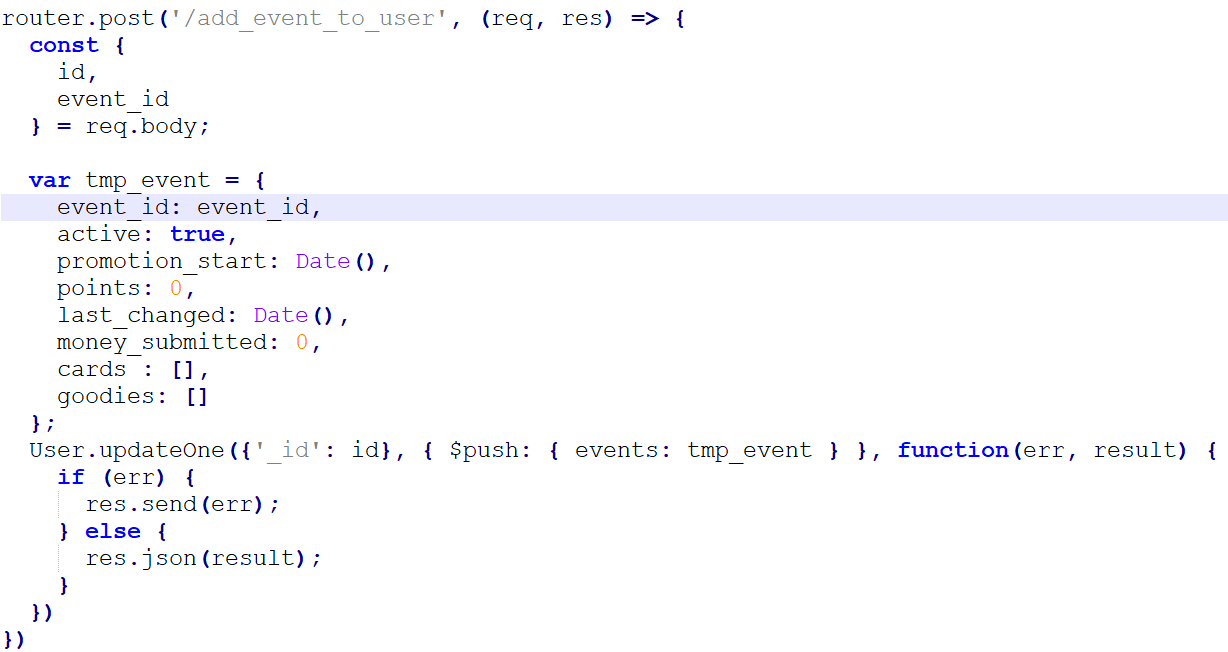
\includegraphics[width=\textwidth]{add_event_to_user.png}
	\caption{'add\_event\_to\_user' Funktion}
\end{figure}	 	
\subsubsection{'create\_user'}
Diese Funktion ist ebenfalls eine Post Funktion welche verwendet wird um einen neuen Promoter oder Administrator in der Datenbank anzulegen. 
Die meisten Daten werden aus der Request gespeichert allerdings werden 3 der benötigten Datenfelder vom Server ausgefüllt und das Password wir durch eine externe Bibliothek gehascht. Danach wir eine temporäres Objekt erstellt welches alle für das erstellen benötigte Daten umfasst. Dieses Objekt wird über Mongoose in die User Kollektion gespeichert. Diese Funktion bildet einen Teil der Grundlage da die EMS Software für eine große Anzahl von Usern ausgelegt ist. 		 		
\begin{figure}[H]
	\centering
	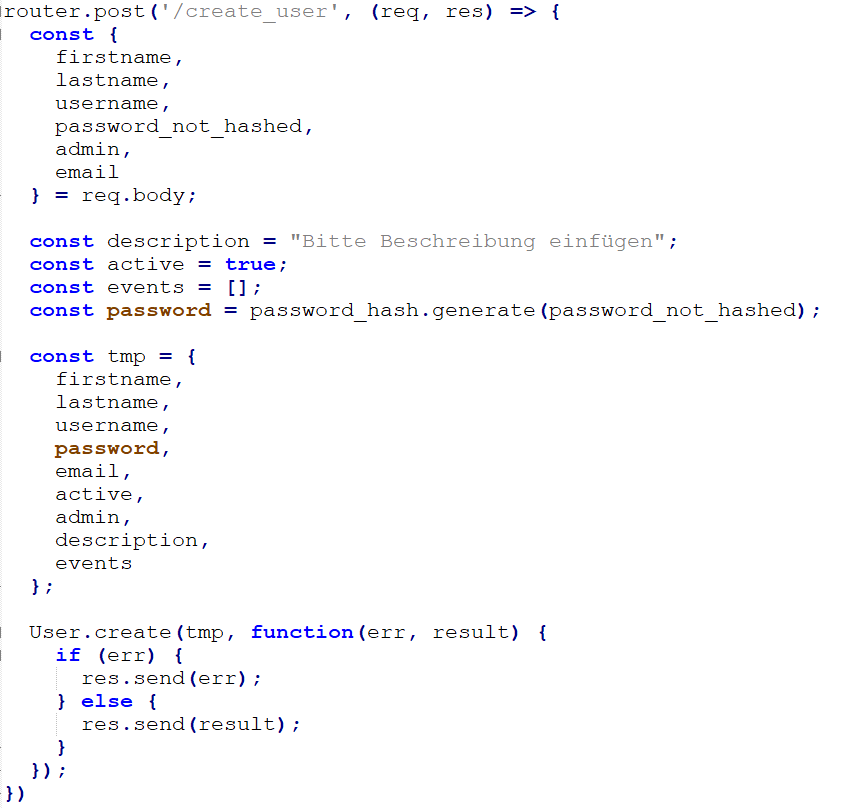
\includegraphics[width=\textwidth]{create_user.png}
	\caption{'create\_user' Funktion}
\end{figure}		 		
\subsubsection{'authenticateToken'}
'authenticateToken' ist eine Middleware welche vor dem ausführen sämtlicher Funktion überprüft ob im Kopf der Anfrage ein gültiger JWS-Token mitgeschickt wurde. Falls ein ungültiger oder falscher Token mitgeschickt wurde wird der Vorgang abgebrochen und eine Fehlermeldung an das Frontend gesendet. Wird ein gültiger Token mitgeschickt wird die Anfrage nach der Überprüfung wie gewollt ausgeführt. Diese Zwischensoftware hilft mit der Sicherheit der Website da keine Anfragen direkt an den Server geschickt werden können ohne das sie von einem eingeloggten User oder Administrator stammen. 		 		
\begin{figure}[H]
	\centering
	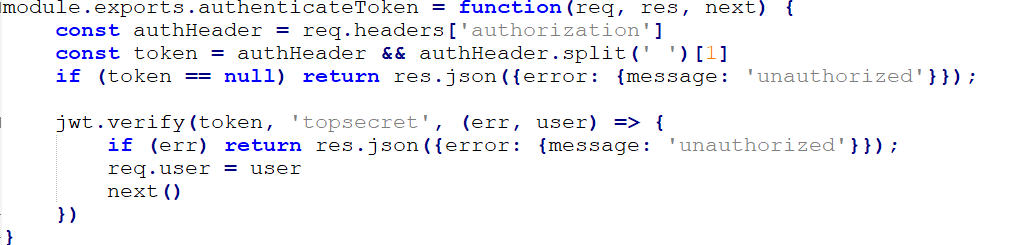
\includegraphics[width=\textwidth]{authentication_middleware.png}
	\caption{'authentication' Middleware}
\end{figure}